% this is Advances in Astronomy and Space Physics tex-sample
% the following preamble cannot be changed accept extension of the packages list; 
% new commands for your own abbreviations can also be added here 
\documentclass[a4paper]{article}
\usepackage{epsfig,amsmath,amsfonts,amssymb,setspace,multirow,textcomp}
\usepackage[T1]{fontenc}
\usepackage[polish]{babel}
\usepackage[utf8]{inputenc}
\usepackage{hyperref}
\textheight 23cm \textwidth 18cm \hoffset= 0mm \voffset= 0cm
\topmargin -1cm \oddsidemargin -8mm \evensidemargin 0mm \columnsep = 4ex
\pagestyle{myheadings}
\renewcommand{\abstractname}{}
\renewcommand{\refname}{\sc references}
\renewcommand{\figurename}{Fig.}
\makeatletter
\renewcommand{\@oddhead}{\textit{Advances in Astronomy and Space Physics} \hfil}
\renewcommand{\@evenfoot}{\hfil \thepage \hfil}
\renewcommand{\@oddfoot}{\hfil \thepage \hfil}
\makeatother
\let\oldthebibliography=\thebibliography
\let\endoldthebibliography=\endthebibliography
\renewenvironment{thebibliography}[1]{\begin{oldthebibliography}{#1}\setlength{\parskip}{0ex}\setlength{\itemsep}{0ex}}{\end{oldthebibliography}}
% end of preamble

\begin{document}
\fontsize{11}{11}\selectfont % the font size cannot be changed in any case!
%  insert your title, authors information and text instead of the one provided below
\title{Signatures of UV radiation around low-mass protostars in Serpens}
\author{\textsl{A.~Mirocha$^{1,}^{2}$, A.~Karska$^{2}$, L.\,E.~Kristensen$^{3}$, M.\,Gronowski$^{4}$, M.\,Figueira$^{5}$, M.\, Gładkowski$^{2,}^{6}$}, \\  \textsl{M.\,Żółtowski$^{7}$, Ł.Tychoniec$^{8}$}}
\date{\vspace*{-6ex}}
\maketitle
\begin{center} {\small $^{1}$ Astronomical Observatory of the Jagiellonian University, ul. Orla 171, 30-244 Kraków, Poland\\
$^{2}$Centre for Astronomy, Faculty of Physics, Astronomy and Informatics, Nicolaus Copernicus University, ul. Grudziądzka 5, 87-100 Toruń, Poland\\
$^{3}$Centre for Star and Planet Formation, Niels Bohr Institute and Natural History Museum of Denmark, University of Copenhagen, Øster Voldgade 5-7, DK-1350 Copenhagen K, Denmark\\
$^{4}$Institute of Physical Chemistry Polish Academy of Sciences, ul. Kasprzaka 44/52, 01-224 Warszawa, Poland\\
$^{5}$National Centre for Nuclear Research, ul. Pasteura 7, 02-093 Warszawa, Poland\\
$^{6}$Nicolaus Copernicus Astronomical Center, ul. Rabiańska 8, 87-100 Toruń, Poland\\
$^{7}$University of Le Havre, Laboratoire Ondes et Milieux Complexes, UMR CNRS 6294,75 Rue Bellot, 76600 Le Havre, France\\
$^{8}$Leiden Observatory, Leiden University, P.O. Box 9513, NL-2300RA Leiden, The Netherlands\\
{\tt amirocha@doctoral.uj.edu.pl}}
\end{center}

\begin{abstract}
A new-born protostar forms in a dense core deep inside a molecular cloud. The molecular cloud is characterised by high extinction in the optical range so observations at long wavelengths are necessary. In particular, submillimetre spectra include rotational lines of key molecules which are useful tracers of physics and chemistry around low-mass protostars. HCN, CN, and CS emission is modelled using the radiative transfer code RADEX to determine the gas physical conditions and molecular abundances. This information provides input parameters to use in an astrochemical model in order to characterise the strength of the UV radiation. Thus, we gain new understandings of chemical and physical processes around low-mass protostars.\\[1ex]
{\bf Key words:} stars: formation, ISM: individual objects: Serpens Main, ISM: molecules
\end{abstract}

\section*{\sc introduction}
\indent \indent New discoveries of extrasolar planets trigger questions about star and planet formation and composition. Detailed studies on the earliest stages of stellar evolution are necessary in order to understand these phenomena. Protostars are formed in dense cores inside a molecular cloud. They can be split by their bolometric luminosity for: low-mass protostars ($L_{\mathrm{bol}} < 10^2 \, L{_\odot}$), intermediate-mass protostars ($10^2 \, L{_\odot} - 10^4 \, L{_\odot}$) and high-mass protostars ($L_{\mathrm{bol}} > 10^4 \, L{_\odot}$). The earliest phases of star formation are characterised by gas and dust accretion from an envelope and bipolar, collimated outflows which transport molecular gas from the dense core (\cite{arce2006}). Protostars interact with their surroundings, changing the chemical and physical properties of the matter in which the stars and planets form. In this turbulent environment, an energetic electromagnetic radiation, such as ultraviolet or X-rays, is produced which causes the ionisation of young stellar objects' environment (\cite{stauber2007}). The UV radiation around massive protostars is estimated at 20-600 times higher than average in the interstellar medium (\cite{benz2016}). The strength of the UV radiation around less massive young stellar objects is still a matter of debates. 

\indent \indent The Serpens molecular cloud is characterised by a large sample of known protostars (\cite{evans2009}). At a distance of 436 $\pm$ 9 pc (\cite{ortiz2017}) it is one of the largest clouds containing low-mass protostars within 500 pc. The Serpens Main region is located in the northern part of the cloud. There are several low-mass protostars at the very early stage of their evolution. The initial identification of the protostars was obtained in the submillimetre range, hence the objects got numbered by their submillimetre luminosity with the SMM prefix. 

\section*{\sc observations}

\indent \indent The observations were obtained with the IRAM 30 telescope between 14th and 17th of July 2009 in good weather conditions. The observations were conduducted with the Eight MIxer Receiver (EMIR) in E090 band and VESPA correlator as the backend which allows obtaining spectra of the targeted lines: HCN, CN, CS and their isotopologues. Two on-the-fly maps of the Ser-SMM1 region (centered at $\alpha_\mathrm{J2000}$ = 18$^h$29$^m$49.6$^s$, $\delta_\mathrm{J2000}$ = +01$^{\circ}$15$^{\prime}$20.5$^{\prime\prime}$) and the Ser-SMM3/Ser-SMM4 region (centered at $\alpha_\mathrm{J2000}$ = 18$^h$29$^m$56.6$^s$, $\delta_\mathrm{J2000}$ = +01$^{\circ}$14$^{\prime}$00.3$^{\prime\prime}$) were obtained. Position-switching mode was chosen. The beam size varies from 14$^{\prime\prime}$ for H$^{13}$CN $J=2-1$ to 29 arcsec for H$^{13}$CN $J=1-0$. The observation summary is shown in Tab.\,\ref{tab:1}.
\begin{table}
\caption{Overview of the observations}             % title of Table
\label{tab:1}      % is used to refer this table in the text
\centering                          % used for centering table
\begin{tabular}{r r r r r}        % centered columns (4 columns)
\hline\hline                 % inserts double horizontal lines
Mol. & Trans. & $\nu$ & Beam size & Beam eff.\\
 & & (GHz) & ($^{\prime\prime}$) & $\eta_\mathrm{MB}$\\
\hline                        % inserts single horizontal line
HCN & $1-0$ & 88.631602 & 28 & 0.81\\
CN & $1-0$ & 113.494921 & 22 & 0.78\\
CS & $3-2$ & 146.969029 & 16 & 0.74\\
C$^{34}$S & $3-2$ & 144.617109 & 16 & 0.74\\
H$^{13}$CN & $1-0$ & 86.342274 & 29 & 0.81\\
H$^{13}$CN & $2-1$ & 172.677881 & 14 & 0.68\\
\hline                                   
\end{tabular}
\begin{flushleft}
Beam sizes and efficiencies are taken from \url{http://www.iram.es/IRAMES/mainWiki/Iram30mEfficiencies}
\end{flushleft}
\end{table}

\section*{\sc results and conclusions}
\indent \indent The HCN molecule photodissociates into CN radical in the presence of the UV radiation while CN itself is less sensitive to photodissociation. Thus, the CN/HCN ratio is widely used as a tracer of the ultraviolet radiation (e.g. \cite{fuente1995},  \cite{chapillon2012}, \cite{riaz2018}). Fig.\,\ref{fig1} shows CN $J=1-0$ and HCN $J=1-0$ integrated intensities ratio, performed above a $3\sigma$ level. In the studied region the highest CN/HCN ratio is co-spatial with more evolved protostars: SMM5 and SMM6. These results show that the CN/HCN ratio can be a good tracer of more evolved protostars independently of a SED analysis. The HCN emission dominates toward molecular outflow positions as well as in denser regions with a large concentration of protostars, where the energetic radiation is mostly absorbed by the dust.

\begin{figure}[!h]
\centering
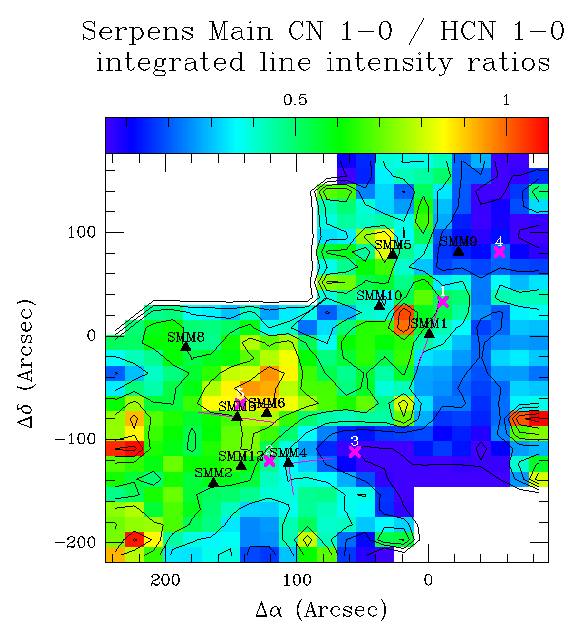
\epsfig{file = serpens_cn10_divided_hcn10.eps,width = 0.5\linewidth}
\caption{Emission of the CN/HCN ratio in the Serpens Main region. Black triangles show the positions of the protostars, whereas black lines show the associated outflow directions. Outflow positions are displayed as purple crosses. The map is centered at the SMM1 position ($\alpha_\mathrm{J2000}$ = 18$^h$29$^m$49.6$^s$, $\delta_\mathrm{J2000}$ = +01$^{\circ}$15$^{\prime}$20.5$^{\prime\prime}$).}
\label{fig1}
\end{figure}

\indent \indent The CN, HCN and CS abundances can be calculated based on the intensities of the observed molecular lines using the RADEX radiative transfer code (\cite{tak2007}). We prepared the sets of RADEX models assuming a kinetic temperature of 50 K and hydrogen densities varying from $10^3$ to $10^6$ cm$^{-3}$. Both CN and HCN $J=1-0$ lines are optically thick with similar optical depths. Even though the absolute column densities may be underestimated, it should not affect the relative N(CN)/N(HCN). The CN/HCN ratio around low-mass protostars varies between 1 and 10 regardless of molecular hydrogen density. The CN/CS ratio varies between 10 and 30 for all of the protostars positions, while the CS/HCN ratio ranges from 0.1 to 0.3. An example of set of models is shown in Fig.\,\ref{fig2}.

\begin{figure}[!h]
\centering
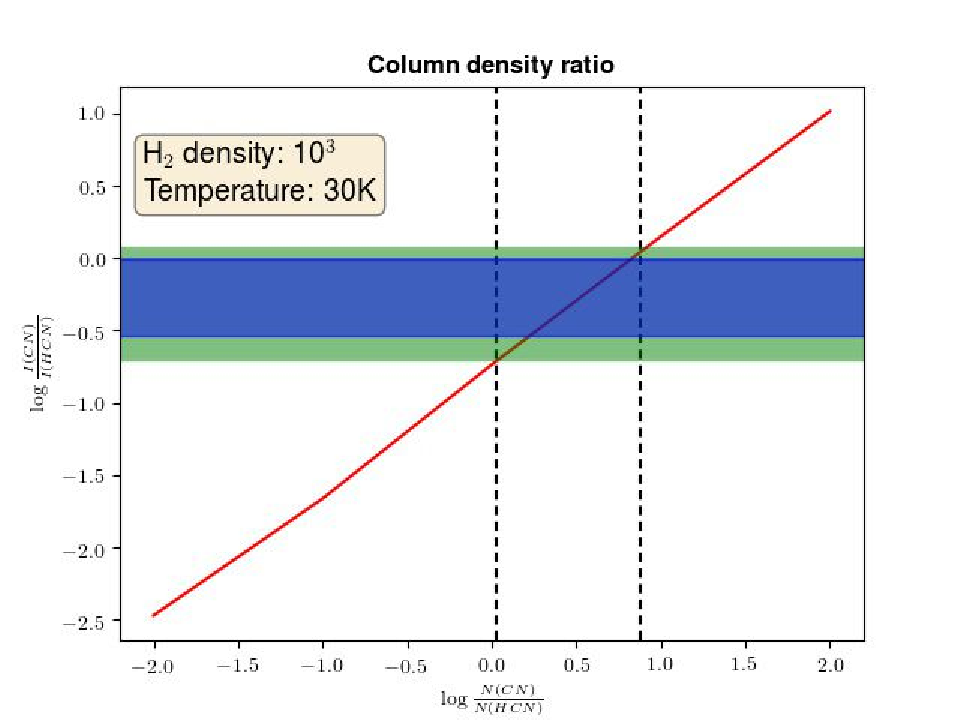
\includegraphics[height=7cm]{radex.jpg}
\caption{N(CN)/N(HCN) column density ratio for $n_\mathrm{H_2} = 10^5$ cm$^{-3}$ and $T_\mathrm{kin} = 50$ K (red line). The observed line intensity ratio is plotted in blue (protostars positions) and green (all positions).}\label{fig2}
\end{figure}

\indent \indent The astrochemical model of Nahoon (\cite{wakelam2012}) together with kida.uva.2014 database (\cite{wakelam2015}) were used in modeling the chemical evolution of the cloud. The astrochemical database kida.uva.2014 contains a list of reactions together with parametrised reaction rate constants. A reaction rate constant depends on the temperature. However, the chemical evolution depends also on several parameters, including UV radiation flux, the cloud density, and temperature as well as dust grain size and abundance. Our model is nearly pure gas-phase model. Our network contains only two class of grain-related reaction, namely: i) between negatively charge grain and atomic cations ii) between neutral grain and electron. The model was run in two steps. In first, we modeled the dense molecular cloud ($n_\mathrm{HI+2 \dot H_2} = 10^4$ cm$^{-3}$, $T = 10$ K, $A_\mathrm{V}$ = 5 mag). The abundances of chemicals obtained at time $10^6$ years were a starting point for a set of models differs by temperature, density, and UV field intensities. The abundances ratio of interesting molecules does not change dynamically at low temperatures which allowed us to fix the temperature parameter at 50 K. Comparing the CN/HCN results with similar plots of CN/CS (Fig.\,\ref{fig3} and Fig.\,\ref{fig4}), we restrict the parameter space to very-low-density and weakly irradiated gas. Astrochemical models computed for the CS/HCN ratio show similar behavior. At the protostellar positions high hydrogen densities ($\approx 10^6$ cm$^{-3}$) can be assumed. The models allow estimating the strength of needed UV radiation field to G$_0 \approx 0.03$. 

\begin{figure}[!h]
\centering
\begin{minipage}[t]{.45\linewidth}
\centering
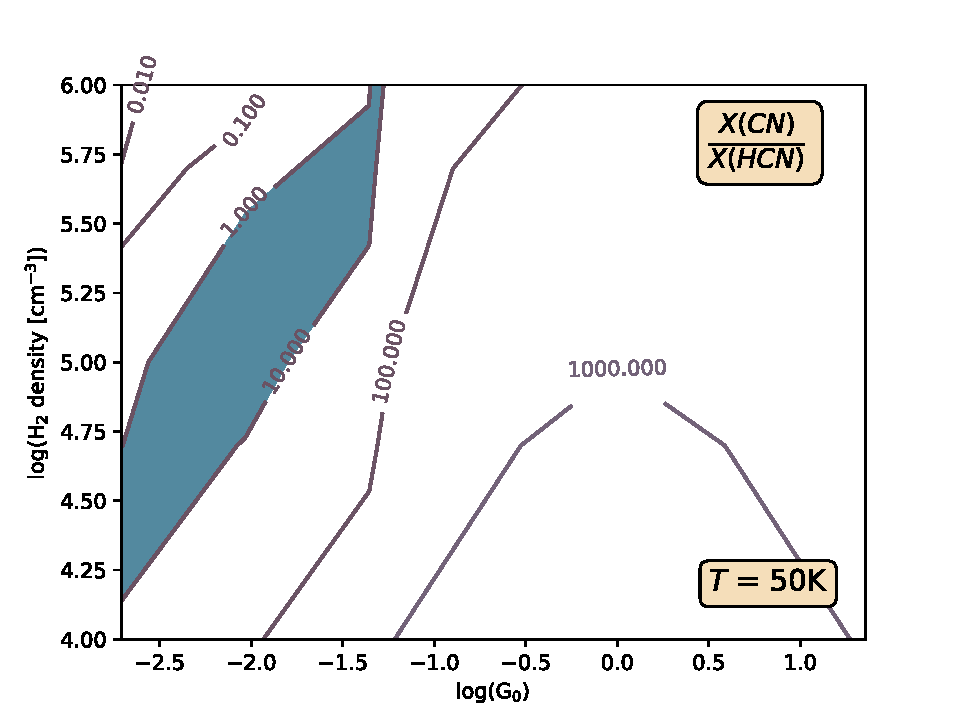
\epsfig{file = CN_HCN.pdf,width = 1\linewidth}
\caption{Contour plot of Nahoon sets of models of CN/HCN abundance ratios with T = 50 K against UV radiation flux (G$_0$ parameter) and hydrogen densities. The observational abundances ratio is represented by the blue area. G$_0$ parameter describes the average UV flux in the ISM of the solar neighbourhood (10$^8$ photons cm$^{−2}$ s$^{−1}$). An additional UV radiation of a few hundredth of the average interstellar UV radiation flux is enough to cover the observations in wide range of total hydrogen densities.}\label{fig3}
\end{minipage}
\hfill
\begin{minipage}[t]{.45\linewidth}
\centering
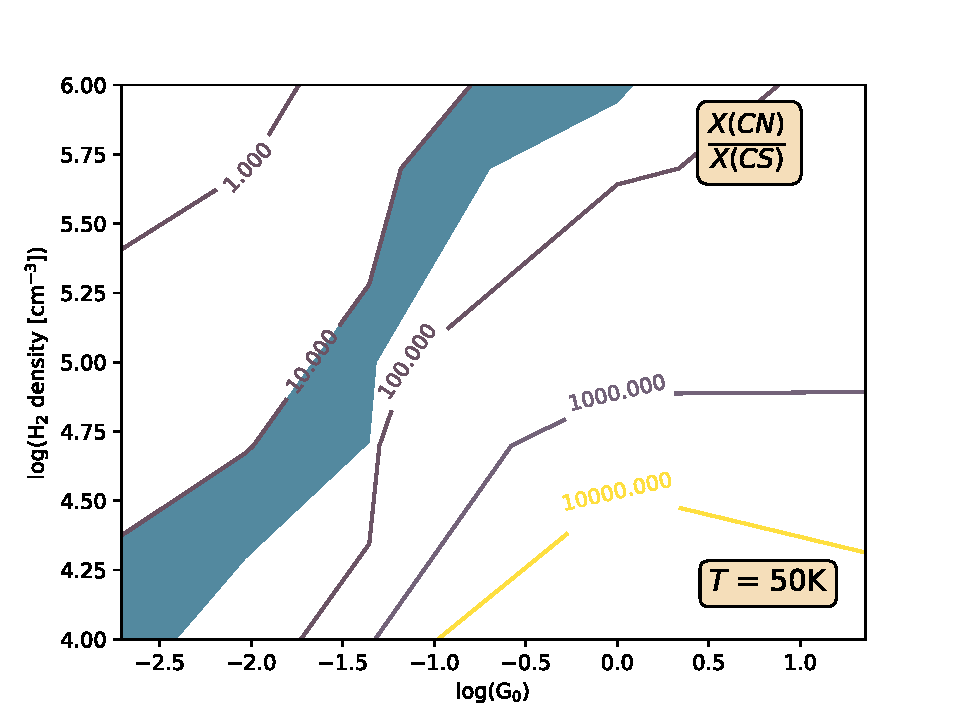
\epsfig{file = CN_CS.pdf,width = 1\linewidth}
\caption{Similar to Fig.~\ref{fig3} but for CN/CS abundances ratios.}\label{fig4}
\end{minipage}
\end{figure}

\indent \indent The astronomical model of Nahoon shows that there is non-zero UV radiation in the gas of 50 K at the positions of low-mass protostars. An additional radiation source of a few hundredth of the average interstellar UV radiation field is required to explain the observational ratios.

\section*{\sc acknowledgement}
\indent \indent AM, AK and MG acknowledge support by the Polish National Science Center grant 2016/21/D/ST9/01098. The research was conducted as a part of the InterAPS project of the Polish National Agency of Academic Exchange.\\
This work is based on observations carried out with the IRAM 30m telescope. IRAM is supported by INSU/CNRS (France), MPG (Germany) and IGN (Spain). \\
This research has made use of data from the Herschel Gould Belt survey (HGBS) project (http://gouldbelt-herschel.cea.fr). The HGBS is a Herschel Key Programme jointly carried out by SPIRE Specialist Astronomy Group 3 (SAG 3), scientists of several institutes in the PACS Consortium (CEA Saclay, INAF-IFSI Rome and INAF-Arcetri, KU Leuven, MPIA Heidelberg), and scientists of the Herschel Science Center (HSC).

% read the instructions for the 
\begin{thebibliography}{10}
{\small
\bibitem{arce2006} Arce, H. G. \& Sargent, A. I. 2006, ApJ, 646, 1070
\bibitem{benz2016} Benz, A. O., Bruderer, S., van Dishoeck, E. F.;, et al. 2016, A\&A, 590, 105
\bibitem{chapillon2012} Chapillon, E., Guilloteau, S., Dutrey, A., et al. 2012, A\&A, 537, A60
\bibitem{evans2009} Evans, Neal J., I., Dunham, M. M., Jørgensen, J. K., et al. 2009, ApJS, 181, 321
\bibitem{fuente1995} Fuente, A., Martin-Pintado, J., \& Gaume, R. 1995, ApJ, 442, L33
\bibitem{ortiz2017} Ortiz-León, G. N., Dzib, S. A., Kounkel, M. A., et al. 2017, ApJ, 834, 143
\bibitem{riaz2018} Riaz, B., Thi, W. F., \& Caselli, P. 2018, MNRAS, 481, 4662
\bibitem{stauber2007} Stäuber, P., Benz, A. O., Jørgensen, J. K., et al. 2007, A\&A, 466, 977 
\bibitem{tak2007} van der Tak, F. F. S., Black, J. H., Schöier, et al. 2007, A\&A, 468, 627
\bibitem{wakelam2012} Wakelam, V., Herbst, E., Loison, J. C., et al. 2012, ApJS, 199, 21
\bibitem{wakelam2015} Wakelam, V., Loison, J. C., Herbst, E., et al. 2015, ApJS, 217, 7
}
\end{thebibliography}
\end{document}
